% main.tex -- draft for IEEE Transactions on Computer-Aided Design of Integrated Circuits and Systems.
% Build: tectonic -X compile main.tex   (or pdflatex + bibtex, twice).
% figs/lp_cartoon.tex is generated: python3 gen/lp_cartoon.py (a toy of the geometry LP, solved, and drawn
% with its real offsets and dual values).
%
% Open items for the author (also marked \TODO{} in the text where they show):
%  - re-run the Zynq ladder on today's make_bench build (these numbers are from the first build);
%  - a per-rung table of crossings, triples and solve time (whole_solve prints them);
%  - a measured benchmark of the dual LP against the primal (the 6x is a single measurement);
%  - an external baseline (a heuristic escape + layer-assignment planner of the Ozdal-Wong / Wu et al. kind,
%    re-implemented on these benches and routed through the same router);
%  - the synthetic buses against their known optima, for the whole route;
%  - check every refs.bib entry marked VERIFY.
\documentclass[journal]{IEEEtran}
\usepackage[cmex10]{amsmath}
\usepackage{amssymb}
\usepackage{graphicx}
\usepackage{booktabs}
\usepackage{cite}
\usepackage{url}
\usepackage{xcolor}
\usepackage{tikz}
\usetikzlibrary{arrows.meta,positioning,calc}

\newtheorem{lemma}{Lemma}
\newtheorem{proposition}{Proposition}
\newcommand{\TODO}[1]{\textcolor{red}{[TODO: #1]}}
\definecolor{Fcu}{RGB}{200,60,60}
\definecolor{Bcu}{RGB}{50,100,200}

\begin{document}

\title{Whole-Route Planning of a Memory Bus Between Two BGAs: Via-Optimal Crossings and Layer Changes, Negotiated to DRC-Clean Copper}

\author{Andrew~Haas%
\thanks{A. Haas is a Professor in the Department of Physics, New York University, New York, NY 10003 USA (e-mail: andy.haas@nyu.edu).}%
\thanks{The software, the benches and the recipes that reproduce every number in this paper are open source~\cite{krt}.}}

\markboth{IEEE Transactions on Computer-Aided Design of Integrated Circuits and Systems}%
{Haas: Whole-Route Planning of a Memory Bus Between Two BGAs}

\maketitle

\begin{abstract}
Routing the bus between a processor and its DRAM remains largely manual in printed circuit board (PCB) design, and published algorithms optimize proxies such as crossing or layer counts at the planning stage. We present a router that plans every lane of a two-layer BGA-to-BGA bus completely before any copper is laid, and carries the plan to finished, design-rule-clean copper. Its core is an exact constraint-programming model that chooses, for all lanes at once, where each necessary crossing occurs, the order of the crossings (consistent with a wiring diagram of the lanes' permutation by a rule over every triple of lanes), and where each lane changes layer, with via room and spacing; it proves the fewest vias within the model. The model reads surprisingly naturally as a problem in physics---worldlines, frustrated Ising spins and contact forces---and the connections proved of practical use. A linear program then places the lanes in millimetres; the constraints it must violate return to the model as cuts, and audit findings as negotiated congestion prices, until the plan passes every rule of the production router. The escapes at both arrays are chosen by the same objective, and differential pairs are planned with their polarity at each end, with an automatic via crossover where the ends disagree. On two public boards, an Allwinner H3 and a Zynq-7020 each to a DDR3 device, the router completes every rung of a ladder of up to 51 nets connected and DRC-clean, never with more vias than the human designer (80 against 88 on the H3, 58 against 103 on the Zynq) and always with less copper.
\end{abstract}

\begin{IEEEkeywords}
Printed circuit board, bus routing, escape routing, topological via minimization, layer assignment, constraint programming, linear programming, differential pairs, DDR.
\end{IEEEkeywords}

\section{Introduction}
\IEEEPARstart{A}{} memory bus is the densest wiring on most processor boards: tens of nets leave a ball grid array (BGA) in a fixed order, arrive at another in a different order, and must cross one another on the way. On a two-layer region every crossing forces one of the two nets onto the other layer there, and every layer change is a via---a drill, an annular ring that blocks both layers, and a discontinuity in the signal path. Designers spend days on such a bus, and commercial tools approach it interactively: the designer sketches the flow, and the tool fills it in.

The literature treats the problem in stages---escape routing, simultaneous escape routing, bus planning and layer assignment (Section~\ref{sec:related})---each optimizing a proxy such as crossings, layers or a planned via count, evaluated against other planners on industrial cases that cannot be reproduced. Whether a plan can be laid in copper at the board's clearance, and how its via count compares with a designer's, are left open.

This paper starts from one observation: \emph{the ends decide the braid}. Once each net's escape at the source and destination is fixed, the orders of those escapes around the two arrays fix which pairs of nets must cross. What remains free is where each crossing happens, in what order the crossings occur, and where each lane changes layer. These choices interact---a via placed to serve one crossing serves or spoils the next, and two vias need room from each other and from every lane passing by---so we decide all of them at once, for every lane, before anything is routed. The contributions are:
\begin{enumerate}
\item An exact constraint-programming (CP) model of the whole route (Section~\ref{sec:solve}) that chooses crossing positions, their order, and every lane's layer changes jointly. Its consistency rule over triples of lanes admits exactly the orders that a wiring diagram of the lanes' permutation can realize. The model proves the fewest vias within its scope.
\item A realization of the plan in board geometry (Section~\ref{sec:copper}): an elastic linear program whose violated constraints return to the CP model as cuts, a snap onto the production router's grid, and an audit against the router's own rules, closed in a negotiation loop that also feeds findings at the ends back to the choice of escapes (Section~\ref{sec:ends}).
\item Differential pairs planned as single lanes with a polarity (handedness) at each end, and an automatic via crossover that swaps P and N where the two ends disagree.
\item An evaluation on two public boards against the human layouts, graded on finished copper by independent design-rule and connectivity checks (Section~\ref{sec:results}).
\end{enumerate}

The models have a surprisingly natural reading in physics. Read along the route, each lane is the worldline of a particle in one space and one time dimension, and each crossing a scattering event; the triple rule that keeps the crossings consistent is the Yang--Baxter relation of three strands. Each worldline carries an Ising spin, its layer, which must disagree with its partner's at every crossing: a via is a domain wall, and frustration is what forces vias. Once the discrete choices are made, placing the lanes is a problem in statics---strings under tension, held apart by struts and walls---whose contact forces are the linear program's dual variables.

\section{Related Work}
\label{sec:related}
\emph{Topological via minimization.} Given the nets' topology, choosing layers to minimize vias is classical. Hsu~\cite{hsu1983} decoupled topology from geometry and assigned layers by a maximum cut; Marek-Sadowska~\cite{marek1984} showed the unconstrained problem NP-complete, and Sarrafzadeh and Lee~\cite{sarrafzadeh1989} gave a polynomial algorithm for nets between two shores, where the problem reduces to covering a permutation graph. Exact and multilayer variants followed~\cite{rim1989,cong1991}; the constrained problem with fixed wire geometry is NP-complete~\cite{naclerio1989} and, on planar instances, a maximum cut that Barahona \emph{et al.}\ solved with the same code as Ising spin-glass ground states~\cite{barahona1988}. These formulations have no geometry: vias need no room, crossings have no position, and the result is never routed.

\emph{PCB escape and bus routing.} Ozdal and Wong chose escape patterns at both ends of a channel jointly to minimize crossings, as a proxy for vias, with a longest-path search for each layer's planar subset and negotiation for the rest~\cite{ozdal2006ser,ozdal2008via}. Bus sequencing, planning and layer assignment for dense boards followed~\cite{kong2007,kong2009,wu2013,yan2009,yan2019,yan2022}, as did exact satisfiability models for escape routing at one array~\cite{luo2008,bayless2016} and escape of differential pairs~\cite{yan2010diff}. Most recently, Wu \emph{et al.}~\cite{wu2026} unified the escape and area regions in one circle model, searched escape orders by simulated annealing, and split unassigned nets with vias, reporting 40.9\% fewer planned vias than a two-phase baseline. All of this work stops at a plan and is evaluated against other planners on private cases.

\emph{Topology, then geometry.} Rubber-band routers~\cite{dai1991} and the theory of homotopic routing~\cite{leiserson1985,hershberger1994} separate a topological route from its embedding. Negotiated congestion~\cite{mcmurchie1995} prices places that were overused before. Commercial tools route groups of nets inside a user's sketch~\cite{potts2015sketch}. Our loop resembles logic-based and combinatorial Benders decomposition~\cite{hooker2003,codato2006}, but its cuts are heuristic generalizations of a geometric failure, not proofs (Section~\ref{sec:loop}).

\emph{Wiring diagrams.} The admissible orders of the crossings of a permutation are those of the higher Bruhat order $B(n,2)$~\cite{manin1989,ziegler1993}, equivalently signotopes and pseudoline sweeps~\cite{felsner2001}. Integer programs over crossing orders appear in graph drawing~\cite{gronemann2016}, and realizing a wiring diagram with prescribed crossings is NP-complete~\cite{yamanaka2018}. We are not aware of a model that uses this structure to minimize vias jointly with crossing positions and via room.

\section{The Problem and the Frame}
\label{sec:problem}
\subsection{Setting}
A \emph{bench} is a board region holding a source BGA $S$ (the processor) and a destination BGA $D$ (the DRAM), a set of bus nets between them, and everything else---passives, other nets' stubs, the board edge---as fixed obstacles. The region has two signal layers, F and B. Each net leaves $S$ at a \emph{tooth}, the end of a fanout stub from its ball, and arrives at $D$ at a \emph{berth}; each end has a layer. The fanout engine offers every ball a menu of escape moves (a stub on one layer, or a dog-bone via to the other), from which the ends are chosen (Section~\ref{sec:ends}). A differential pair is one \emph{lane} with two legs. Rules are those of the boards' fabrication process: clearance 0.1\,mm, lane track 0.127\,mm, fanout track 0.1\,mm, vias 0.25\,mm with a 0.15\,mm drill, and a routing grid of 0.025\,mm. Two neighbouring lanes on one layer must lie at least a \emph{bar} of 0.232\,mm apart, centre to centre.

The objective is lexicographic: first, the number of nets with more than two vias on the board (their stubs' vias included, a pair's barrels counted per leg); second, the number of vias; third, a congestion tie-break. The result must be routed by the production router, connected, and clean under a design-rule check (DRC) at the board's clearance.

\subsection{The frame and the route coordinate}
The frame is read off the board alone. A straight \emph{trunk} runs from the pad box of $S$ through that of $D$; a \emph{ring} follows the octilinear hull of $D$'s pads and stubs around each of its two long faces. Unrolling the perimeter of $S$ from a cut on its far face gives the \emph{launch order} $\lambda$ of the teeth; unrolling that of $D$ from a cut at the widest gap on its far face gives the \emph{berth order} $\varphi$. Every lane's route is then one scalar coordinate $u$: along the trunk from its tooth, then along its ring to its berth. We discretize $u$ on a grid $G$ of a fifth of the least planned lane pitch $p=0.252$\,mm, about 0.05\,mm.

A pair of lanes $(a,b)$ with $\lambda(a)<\lambda(b)$ is \emph{inverted} if $\varphi(a)>\varphi(b)$. Every inverted pair must cross; in our model it crosses exactly once, and no other pair crosses. The set $I$ of inverted pairs is the inversion set of the permutation $\pi$ that takes launch order to berth order (Fig.~\ref{fig:braid}).

\begin{figure}[t]
\centering
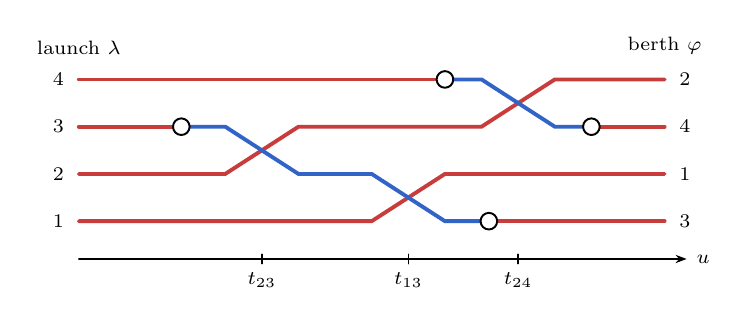
\begin{tikzpicture}[x=0.93cm,y=0.6cm,line width=1.4pt,line cap=round]
\draw[Fcu] (0,0)--(4,0)--(5,1)--(8,1);
\draw[Fcu] (0,1)--(2,1)--(3,2)--(5.5,2)--(6.5,3)--(8,3);
\draw[Fcu] (0,2)--(1.4,2);
\draw[Bcu] (1.4,2)--(2,2)--(3,1)--(4,1)--(5,0)--(5.6,0);
\draw[Fcu] (5.6,0)--(8,0);
\draw[Fcu] (0,3)--(5.0,3);
\draw[Bcu] (5.0,3)--(5.5,3)--(6.5,2)--(7.0,2);
\draw[Fcu] (7.0,2)--(8,2);
\foreach \p in {(1.4,2),(5.6,0),(5.0,3),(7.0,2)} \draw[line width=0.7pt,fill=white] \p circle (3pt);
\foreach \y/\l in {0/1,1/2,2/3,3/4} \node[font=\scriptsize,left] at (-0.05,\y) {$\l$};
\foreach \y/\l in {0/3,1/1,2/4,3/2} \node[font=\scriptsize,right] at (8.05,\y) {$\l$};
\node[font=\scriptsize,above] at (0,3.3) {launch $\lambda$};
\node[font=\scriptsize,above] at (8,3.3) {berth $\varphi$};
\draw[-{Stealth[length=4pt]},line width=0.5pt] (0,-0.8)--(8.3,-0.8) node[right,font=\scriptsize]{$u$};
\foreach \x/\l in {2.5/{t_{23}},4.5/{t_{13}},6/{t_{24}}} {
  \draw[line width=0.5pt] (\x,-0.9)--(\x,-0.7);
  \node[below,font=\scriptsize] at (\x,-0.85) {$\l$};}
\end{tikzpicture}
\caption{Four lanes as a wiring diagram along the route coordinate $u$. The berth order is $\pi=(3,1,4,2)$, so the inverted pairs $\{2,3\},\{1,3\},\{2,4\}$ must each cross once. On the triple $(1,2,3)$ only $\{1,3\}$ and $\{2,3\}$ are inverted, so the triple rule forces $t_{23}<t_{13}$. Red is F, blue is B; circles are vias. Crossing lanes are on different layers. Lane 3 serves its two F partners in one excursion to B, and lane 4 serves one: four vias, equal to the floor $2(K-\mathrm{LIS}(\pi))=2(4-2)$ of Lemma~\ref{lem:floor}.}
\label{fig:braid}
\end{figure}

\subsection{Two bounds}
\begin{lemma}[Floor]
\label{lem:floor}
If both ends of every lane are on F, any routing needs at least $2(K-\mathrm{LIS}(\pi))$ vias, where $\mathrm{LIS}$ is the length of the longest increasing subsequence.
\end{lemma}
\begin{IEEEproof}
Lanes that never change layer stay on F and so cannot cross one another; they form an increasing subsequence of $\pi$. Every other lane leaves F and returns, at least two vias.
\end{IEEEproof}
The floor is the classical maximum planar subset~\cite{supowit1987} in the two-shore case~\cite{sarrafzadeh1989}, and it is weak: lanes that leave F also cross one another, and an excursion to B cannot serve a crossing with a partner that is itself on B. For a uniformly random permutation the LIS grows as $2\sqrt{K}$, with Tracy--Widom fluctuations of order $K^{1/6}$~\cite{baik1999}---the statistics of the KPZ class of growth processes~\cite{prahofer2000}. Real buses are structured rather than random, but the scaling is a yardstick for how the floor grows with the width of a bus. The next lemma counts a lane's vias exactly, given its partners.

\begin{lemma}[Blocks]
\label{lem:blocks}
Fix the layers of lane $n$'s crossing partners at their crossings, in the order the crossings occur along $n$, and let both ends of $n$ be on F. The fewest layer changes of $n$ is twice the number of maximal runs of consecutive partners that are on F.
\end{lemma}
\begin{IEEEproof}
At each crossing $n$ must be on the partner's opposite layer: on B across a maximal run of F partners, on F across a run of B partners and at both ends. Each F run therefore needs one change into B and one out, and no change is needed elsewhere.
\end{IEEEproof}
Applied to the partners' layers as laid, Lemma~\ref{lem:blocks} reproduces the via count of all 47 nets examined, both on the human's H3 board and on a board routed by an earlier version of our router: neither places a redundant via. The difficulty is therefore not placing a lane's vias given its partners, but choosing every lane's layers and crossing order together---which is what the whole-route model does.

\section{The Whole-Route Solve}
\label{sec:solve}
One CP-SAT~\cite{cpsat} model decides every crossing and every layer change for all lanes at once (Fig.~\ref{fig:beads}).

\begin{figure}[t]
\centering
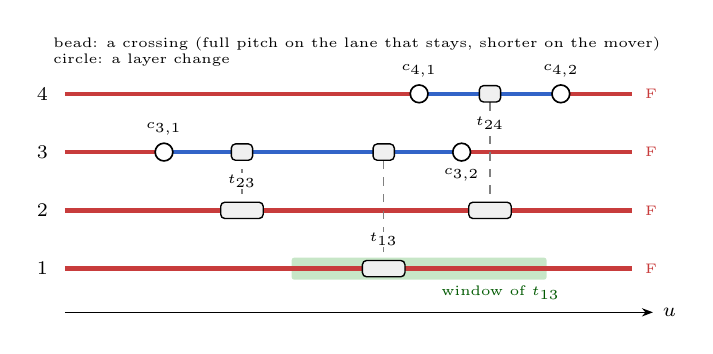
\begin{tikzpicture}[x=0.9cm,y=0.74cm,font=\scriptsize,
  bead/.style={draw=black,fill=gray!12,rounded corners=1.5pt,line width=0.5pt},
  tie/.style={gray,dashed,line width=0.5pt}]
\fill[green!55!black,opacity=0.22,rounded corners=1pt] (3.2,-0.19) rectangle (6.8,0.19);
\node[green!35!black,font=\tiny] at (6.15,-0.42) {window of $t_{13}$};
\draw[Fcu,line width=1.6pt] (0,0)--(8,0);
\draw[Fcu,line width=1.6pt] (0,1)--(8,1);
\draw[Fcu,line width=1.6pt] (0,2)--(1.4,2);
\draw[Bcu,line width=1.6pt] (1.4,2)--(5.6,2);
\draw[Fcu,line width=1.6pt] (5.6,2)--(8,2);
\draw[Fcu,line width=1.6pt] (0,3)--(5.0,3);
\draw[Bcu,line width=1.6pt] (5.0,3)--(7.0,3);
\draw[Fcu,line width=1.6pt] (7.0,3)--(8,3);
\draw[tie] (2.5,1)--(2.5,2);
\draw[tie] (4.5,0)--(4.5,2);
\draw[tie] (6.0,1)--(6.0,3);
\draw[bead] (2.2,0.86) rectangle (2.8,1.14);
\draw[bead] (2.35,1.86) rectangle (2.65,2.14);
\draw[bead] (4.2,-0.14) rectangle (4.8,0.14);
\draw[bead] (4.35,1.86) rectangle (4.65,2.14);
\draw[bead] (5.7,0.86) rectangle (6.3,1.14);
\draw[bead] (5.85,2.86) rectangle (6.15,3.14);
\node[font=\tiny,fill=white,inner sep=0.6pt] at (2.5,1.5) {$t_{23}$};
\node[font=\tiny,fill=white,inner sep=0.6pt] at (4.5,0.5) {$t_{13}$};
\node[font=\tiny,fill=white,inner sep=0.6pt] at (6.0,2.5) {$t_{24}$};
\foreach \p/\l/\w in {(1.4,2)/{c_{3,1}}/above, (5.6,2)/{c_{3,2}}/below, (5.0,3)/{c_{4,1}}/above, (7.0,3)/{c_{4,2}}/above} {
  \draw[line width=0.6pt,fill=white] \p circle (3.2pt);
  \node[font=\tiny,\w=2.5pt] at \p {$\l$};}
\foreach \y/\l in {0/1,1/2,2/3,3/4} {
  \node[left] at (-0.1,\y) {$\l$};
  \node[right,font=\tiny,Fcu] at (8.05,\y) {F};}
\node[font=\tiny,align=left,anchor=south west] at (-0.3,3.3) {bead: a crossing (full pitch on the lane that stays, shorter on the mover)\\circle: a layer change};
\draw[-{Stealth[length=4pt]},line width=0.5pt] (0,-0.75)--(8.3,-0.75) node[right]{$u$};
\end{tikzpicture}
\caption{The whole-route model as beads on tracks, for the four lanes of Fig.~\ref{fig:braid} (all ends on F). Each lane's route coordinate $u$ is a track, drawn in launch order. A crossing variable $t_{ab}$ is one bead that sits on both lanes' tracks at once (dashed tie), and intervals on one track may not overlap; each crossing slides only within its window (green, shown for $t_{13}$). Layer changes $c_{n,k}$ are beads too (circles), and between them a track's colour is its layer. The model requires tied tracks to differ in colour at their bead and each lane's number of changes to have the parity of its end layers, and the triple rule orders $t_{23}$ before $t_{13}$. The solver slides every bead at once and proves the fewest changes.}
\label{fig:beads}
\end{figure}

\emph{Crossings.} For each $(a,b)\in I$ an integer $t_{ab}\in[\ell_{ab},h_{ab}]$ on the grid $G$ is the crossing's position along the route. Its window starts after both lanes have entered the trunk, keeps a margin from both terminals, excludes the band in front of the source face where the teeth stand, and ends at the handoff to the rings unless both lanes share a ring. The \emph{triple rule}: for every $i<j<k$ in launch order,
\begin{itemize}
\item if $ij,ik,jk\in I$: $t_{ij}<t_{ik}<t_{jk}$ or $t_{jk}<t_{ik}<t_{ij}$ (one Boolean);
\item if $ij,ik\in I$ and $jk\notin I$: $t_{ij}<t_{ik}$;
\item if $ik,jk\in I$ and $ij\notin I$: $t_{jk}<t_{ik}$.
\end{itemize}
The case $ij,jk\in I$, $ik\notin I$ cannot occur.
\begin{proposition}
\label{prop:triple}
A linear order of $I$ is the order in which the crossings of some wiring diagram (reduced word) of $\pi$ occur if and only if it satisfies the triple rule.
\end{proposition}
\begin{IEEEproof}[Sketch]
In a wiring diagram two lanes cross only when adjacent, so after any prefix of crossings the lanes stand in the order of some permutation, and the prefix is its inversion set; conversely, if a prefix and its extension by one pair are both inversion sets, that pair is adjacent and can cross next. A set of pairs is an inversion set if and only if, on every triple, it is closed ($ij,jk$ in the set imply $ik$) and co-closed ($ik$ implies $ij$ or $jk$)~\cite{bjorner2005}. Requiring this of every prefix, triple by triple, gives exactly the three cases above.
\end{IEEEproof}
For the longest permutation these are the admissible orders of the higher Bruhat order $B(n,2)$~\cite{manin1989,ziegler1993,felsner2001}. Crossings of disjoint pairs may coincide---they commute---while crossings that share a lane are kept apart by a per-lane no-overlap constraint on intervals of the lane pitch. A Boolean per crossing chooses which lane \emph{stays} and which \emph{moves} across: the stayer's interval is the full pitch, the mover's the shorter footprint of its sweep. The two crossings of a pair lane that pass other lanes in opposite directions are kept a turning run apart.

\emph{Worldlines.} Read $u$ as time and the lane order as position on a line: each lane is then the worldline of a particle in one space and one time dimension, and a crossing is a two-body scattering event. Three mutually crossing lanes can scatter in only two orders, $t_{ij}<t_{ik}<t_{jk}$ or its reverse---the two sides of the Yang--Baxter relation~\cite{yang1967,baxter1972}, or the third Reidemeister move. In an integrable theory the two sides are equal and scattering factorizes~\cite{zamolodchikov1979}; on a board they differ in cost, and the triple rule's Boolean is the solver's choice between them.

\emph{Layer changes.} Each lane $n$ has up to three change positions $c_{n,1..3}$ with activity literals $a_{n,k}$; active changes are ordered and a via's room $D_v$ apart, and their parity is fixed by the ends:
\begin{equation}
\textstyle\bigoplus_k a_{n,k} \;=\; \ell^{S}_n \oplus \ell^{D}_n ,
\end{equation}
where $\ell^S_n,\ell^D_n\in\{0,1\}$ are the end layers. For each crossing $(a,b)$ and each change $k$ of lane $a$, a literal $\beta_{a,k,ab}$ states that the change lies before the crossing, enforced with clearance: $c_{a,k}\le t_{ab}-h$ or $c_{a,k}\ge t_{ab}+h$, where $h$ is the room of both lanes there (wider when the crossing lane is a pair, and dependent on the stay/move choice). The layer of $a$ at the crossing is $\ell^S_a\oplus\bigoplus_k(a_{a,k}\wedge\beta_{a,k,ab})$, and crossing lanes must differ:
\begin{equation}
\textstyle
\ell^S_a\oplus\ell^S_b\oplus\bigoplus_k (a_{a,k}\wedge\beta_{a,k,ab})\oplus\bigoplus_k (a_{b,k}\wedge\beta_{b,k,ab}) \;=\; 1 .
\end{equation}
Changes of lanes that can be neighbours---adjacent in $\lambda$ or $\varphi$, or crossing each other---are staggered along $u$ by $\max(v,\sqrt{v_v^2-p^2})$, so that two vias one pitch $p$ apart across the bus still meet the via-to-via rule $v_v$.

\emph{Spins.} Give each worldline an Ising spin, its layer. Equation~(2) is then a hard antiferromagnetic bond at every crossing, a via is a domain wall along a worldline, and the objective counts domain walls. A cycle of must-differ constraints with an odd number of links cannot be satisfied without a wall---it is frustrated~\cite{toulouse1977}---and frustration is what forces vias. With the crossing order fixed this is the planar spin-glass ground state that Barahona \emph{et al.}\ solved as a maximum cut alongside via minimization~\cite{barahona1988}, and Lemma~\ref{lem:blocks} counts the domain walls of one worldline in the field of its partners. The whole-route solve also chooses the order of the scattering events.

\emph{Built-in cuts.} A lane's changes stay off stretches where its reference path passes within a via's reach of another part's pad or of a foreign net's tooth, and a pair's changes stay off the corners its route is known to turn and out of its end connectors (Section~\ref{sec:pairs}).

\emph{Objective.} With $o_n\ge s_n+\sum_k a_{n,k}-2$ counting the vias of net $n$ beyond two ($s_n$ its stub vias),
\begin{equation}
\min\; W_O\sum_n o_n \;+\; W_V\sum_{n,k} a_{n,k} \;+\; H ,
\end{equation}
with $W_V=10^6$, $W_O=W_V(3K+1)$, and $H$, the history term of Section~\ref{sec:loop}, below one via. Preferring at most two vias per net is a preference, not a cap: a cap is infeasible on many instances.

\emph{Proving it.} CP-SAT runs four workers: two linear-relaxation searches, a core-based search and an objective lower-bound search. The bound-raising workers are essential: CP-SAT's default portfolio left the first solve of the 51-net rung unproved after 421\,s (56 vias against a bound of 40); with them it is proved in 22--37\,s. When they cannot prove a plan, a second run with plan-finding workers starts from the best plan and with the bound as a constraint. A re-solve in the loop only adds cuts and history below a via, so the first solve's optimum is a valid floor for it; adding the floor turned an unproved 193\,s re-solve into a proof in 73\,s. Every budget is a count of deterministic work, never a clock. \emph{Only a plan proved optimal in its vias goes on}; one the search could not prove is no plan.

\emph{Scope.} The proof is relative to the model: the ends are fixed, each inverted pair crosses once (non-reduced braids are excluded), a lane changes layer at most three times (every proved plan we have seen uses at most two), positions lie on $G$, and the loop's cuts are heuristic.

\section{Choosing the Ends}
\label{sec:ends}
Because the ends decide the braid, the escapes at both arrays are chosen with the solve's own objective. For a candidate assignment of teeth and berths we estimate the route's vias from the ends alone:
among lanes whose ends share a layer, inverted pairs on one layer must be separated by lanes that dive, and since their conflict graph is a permutation graph the cheapest cover is the complement of a maximum-weight increasing chain, exact per layer; a lane whose ends differ changes once, and the partners it would meet on the wrong layer form a bipartite graph covered exactly by a minimum cut; conflicts between such lanes are resolved greedily. Congestion adds each lane's load on the trunk (the room its crossings and changes take), priced by the square of its excess over half, and a fifth of a via per trunk crossing. The crossing price exists because the solve's effort follows its crossings, not its vias: at 131 crossings the 35-net rung proved in 10\,s, at 163 in 121\,s; at a twentieth of a via per crossing the 41-net ends stalled, at a fifth they proved in 26--38\,s. The search moves one tooth or berth at a time (ejecting one conflicting lane where needed), then iterates from seeded random kicks; the best few states are re-ranked exactly by the solve's order model without lengths. A board the fanout engine does not lay exactly as asked is discarded and its missed moves are banned.

\emph{Street berths.} A DDR3 package leaves an unpopulated band between its two ball groups. A ball beside it may run into a lane of the band, dive there, and leave along the band on the other layer---as the human does with 20 of its 30 signal vias at the DRAM. Offering such berths cut the 35-net rung's crossings from 162 to 132 and its solve from 121 to 10\,s, at 6 more vias.

\section{From Plan to Copper}
\label{sec:copper}
\subsection{Geometry}
A single linear program places every lane: an offset per lane per column, columns every four grid steps (0.1\,mm) along the trunk and both rings, joined where each lane's trunk ends. Constraints keep each column's lanes in the solve's order on their solved layers, same-layer neighbours a bar apart (slope-corrected by tangent cuts), a via's room around every change (chords of a disc at neighbouring columns), every lane inside the board and off the pad boxes, and turns within 45$^\circ$ per column (per turning run for a pair). Costs are the added length---under-estimated by tangent cuts, so that a small sideways move costs next to nothing and lanes take a \emph{comfortable} pitch where there is room---the bends, and a hinge penalty on neighbours closer than the comfortable pitch. Every hard constraint is elastic, its slack priced at $W_H=10^4$ per millimetre, so the program always has a solution and reports exactly where it had to break a rule.

A second pass holds each lane to one side of every \emph{island}---a part's pads, or several parts no lane can pass between. The choice of side is non-convex, so it is made combinatorially before the pass, by neither the LP nor the CP-SAT model: at each island the lanes, in the order the CP-SAT solve fixed there, are split at the index that the first pass's offsets make cheapest, and the island is inserted into the order at that split. The sides therefore never contradict the crossing plan, and the program stays convex. The constraints paid in the second pass become cuts for the solve: a lane that could not be kept off an island may not cross anyone over the island's span; a change that could not be given its room may not lie there.

The program is large (7\,205 variables and 150\,960 constraints for pass one of the 51-net rung) and has far more constraints than variables, so we pass its dual to HiGHS~\cite{huangfu2018,schork2020} through SciPy~\cite{scipy2020} and read the offsets back as the multipliers of the dual's balance equations; on the 51-net rung's second pass this took 31\,s rather than 188\,s.\TODO{benchmark primal against dual over the ladder.}

\emph{Forces.} The program's optimality conditions are those of a mechanism at rest (Fig.~\ref{fig:lp}). Each lane point is a bead that slides on its column's rail, the length term is a string at unit tension, and the rules are contacts: struts between neighbours, walls at the pads and the board edge. A rule's dual value is the force in its contact, and complementary slackness is the contact law---a strut pushes only while it touches. An elastic rule is a rigid-plastic strut that carries up to $W_H$ and then yields. The static and kinematic theorems of plastic collapse are this duality~\cite{charnes1959}, and the linear program that tests a packing of hard spheres for jamming solves for the same contact forces~\cite{donev2004}. The picture is of practical use. Of the 150\,960 constraints of the 51-net rung only 376 carry a force, and those, with the lanes' pinned ends, determine every offset; the forces name the rules that hold each lane, and the struts that yield at $W_H$ are exactly the constraints returned to the solve as cuts.

\begin{figure}[t]
\centering
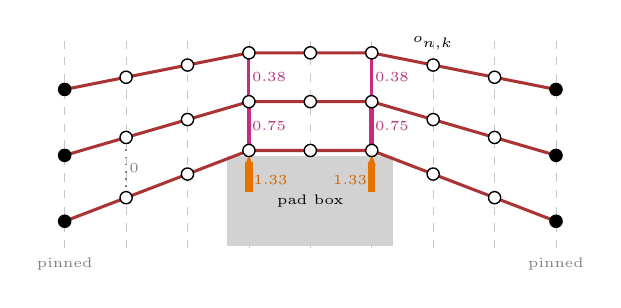
\begin{tikzpicture}[x=0.78cm,y=0.62cm,font=\scriptsize]
\draw[gray!45,dashed,line width=0.3pt] (0,-0.55)--(0,3.8);
\draw[gray!45,dashed,line width=0.3pt] (1,-0.55)--(1,3.8);
\draw[gray!45,dashed,line width=0.3pt] (2,-0.55)--(2,3.8);
\draw[gray!45,dashed,line width=0.3pt] (3,-0.55)--(3,3.8);
\draw[gray!45,dashed,line width=0.3pt] (4,-0.55)--(4,3.8);
\draw[gray!45,dashed,line width=0.3pt] (5,-0.55)--(5,3.8);
\draw[gray!45,dashed,line width=0.3pt] (6,-0.55)--(6,3.8);
\draw[gray!45,dashed,line width=0.3pt] (7,-0.55)--(7,3.8);
\draw[gray!45,dashed,line width=0.3pt] (8,-0.55)--(8,3.8);
\fill[gray!35] (2.65,-0.5) rectangle (5.35,1.33);
\node[font=\tiny] at (4.00,0.41) {pad box};
\draw[Fcu!85!black,line width=1.1pt] (0,0.000)--(1,0.483)--(2,0.967)--(3,1.450)--(4,1.450)--(5,1.450)--(6,0.967)--(7,0.483)--(8,0.000);
\draw[Fcu!85!black,line width=1.1pt] (0,1.350)--(1,1.717)--(2,2.083)--(3,2.450)--(4,2.450)--(5,2.450)--(6,2.083)--(7,1.717)--(8,1.350);
\draw[Fcu!85!black,line width=1.1pt] (0,2.700)--(1,2.950)--(2,3.200)--(3,3.450)--(4,3.450)--(5,3.450)--(6,3.200)--(7,2.950)--(8,2.700);
\draw[magenta!80!black,line width=1.74pt] (3,1.520)--(3,2.380);
\node[magenta!70!black,right,font=\tiny,inner sep=1pt] at (3,1.950) {0.75};
\draw[magenta!80!black,line width=1.12pt] (3,2.520)--(3,3.380);
\node[magenta!70!black,right,font=\tiny,inner sep=1pt] at (3,2.950) {0.38};
\draw[magenta!80!black,line width=1.74pt] (5,1.520)--(5,2.380);
\node[magenta!70!black,right,font=\tiny,inner sep=1pt] at (5,1.950) {0.75};
\draw[magenta!80!black,line width=1.12pt] (5,2.520)--(5,3.380);
\node[magenta!70!black,right,font=\tiny,inner sep=1pt] at (5,2.950) {0.38};
\draw[orange!90!black,line width=2.70pt,-{Stealth[length=4pt]}] (3,0.600)--(3,1.360);
\node[orange!80!black,right,font=\tiny,inner sep=1.5pt] at (3,0.850) {1.33};
\draw[orange!90!black,line width=2.70pt,-{Stealth[length=4pt]}] (5,0.600)--(5,1.360);
\node[orange!80!black,left,font=\tiny,inner sep=1.5pt] at (5,0.850) {1.33};
\draw[gray,dotted,line width=0.6pt] (1,0.553)--(1,1.647);
\node[gray,right,font=\tiny,inner sep=1pt] at (1,1.100) {0};
\filldraw[fill=black,line width=0.5pt] (0,0.000) circle (2.2pt);
\filldraw[fill=white,line width=0.5pt] (1,0.483) circle (2.2pt);
\filldraw[fill=white,line width=0.5pt] (2,0.967) circle (2.2pt);
\filldraw[fill=white,line width=0.5pt] (3,1.450) circle (2.2pt);
\filldraw[fill=white,line width=0.5pt] (4,1.450) circle (2.2pt);
\filldraw[fill=white,line width=0.5pt] (5,1.450) circle (2.2pt);
\filldraw[fill=white,line width=0.5pt] (6,0.967) circle (2.2pt);
\filldraw[fill=white,line width=0.5pt] (7,0.483) circle (2.2pt);
\filldraw[fill=black,line width=0.5pt] (8,0.000) circle (2.2pt);
\filldraw[fill=black,line width=0.5pt] (0,1.350) circle (2.2pt);
\filldraw[fill=white,line width=0.5pt] (1,1.717) circle (2.2pt);
\filldraw[fill=white,line width=0.5pt] (2,2.083) circle (2.2pt);
\filldraw[fill=white,line width=0.5pt] (3,2.450) circle (2.2pt);
\filldraw[fill=white,line width=0.5pt] (4,2.450) circle (2.2pt);
\filldraw[fill=white,line width=0.5pt] (5,2.450) circle (2.2pt);
\filldraw[fill=white,line width=0.5pt] (6,2.083) circle (2.2pt);
\filldraw[fill=white,line width=0.5pt] (7,1.717) circle (2.2pt);
\filldraw[fill=black,line width=0.5pt] (8,1.350) circle (2.2pt);
\filldraw[fill=black,line width=0.5pt] (0,2.700) circle (2.2pt);
\filldraw[fill=white,line width=0.5pt] (1,2.950) circle (2.2pt);
\filldraw[fill=white,line width=0.5pt] (2,3.200) circle (2.2pt);
\filldraw[fill=white,line width=0.5pt] (3,3.450) circle (2.2pt);
\filldraw[fill=white,line width=0.5pt] (4,3.450) circle (2.2pt);
\filldraw[fill=white,line width=0.5pt] (5,3.450) circle (2.2pt);
\filldraw[fill=white,line width=0.5pt] (6,3.200) circle (2.2pt);
\filldraw[fill=white,line width=0.5pt] (7,2.950) circle (2.2pt);
\filldraw[fill=black,line width=0.5pt] (8,2.700) circle (2.2pt);
\node[above,font=\tiny] at (6,3.300) {$o_{n,k}$};
\node[below,font=\tiny,gray] at (0,-0.55) {pinned};
\node[below,font=\tiny,gray] at (8,-0.55) {pinned};
\end{tikzpicture}

\caption{A small instance of the geometry LP, solved. Three lanes on one layer cross nine columns, pinned at both ends (black), and must pass over a pad box. Each lane point slides on its column's rail (dashed); the lanes are strings at unit tension. The rules that bind carry the dual values drawn: the box (orange) pushes the lowest lane up where the lanes bend, and pitch struts (magenta) pass the load up the stack, each carrying exactly the pull of the strings above it. Every other rule carries no force, like the strut near the pins (dotted), which has room to spare. Forces are in units of the string tension.}
\label{fig:lp}
\end{figure}

\subsection{Polish and snap}
The \emph{polish} meets the audit's own measures in board coordinates (pitch, via room, clearance to pads as drawn, turn shapes) by small vertex moves, one linear program per round, with every bar a grid step above the snap's. A lane that cannot be held on its side of an island is flipped, and the geometry runs again.

The \emph{snap} makes the smooth plan octilinear on the router's grid, one lane at a time, by an A$^*$ search in a band around each lane's smooth line that prices length, bends and distance from the line. Pairs go first, moving exactly as the pair router moves (45$^\circ$ turns, a straight run after each turn, a via only on a straight run); they are then held while the polish fits the singles around them. A lane not yet laid keeps a share of every gap---the side of the midline nearer its own line, less half a bar---so lanes laid first cannot take the room later ones need. Two sweeps then lay every lane again against the others' real copper.

\subsection{Differential pairs}
\label{sec:pairs}
A pair is one lane of two slots' width. Its \emph{hand} at an end is the side of its travel on which P lies (the sign of the cross product of the travel direction with the vector from N to P). A pair whose hands at its tooth and berth disagree must swap its legs somewhere; the solve then requires it to change layer at least once, and the snap lays a \emph{crossover} at its first dive, as a designer would: the first leg jogs out at 45$^\circ$ to its barrel and dives, the second jogs at 45$^\circ$ over the first leg's new-layer segment to a barrel just beyond and returns to its line. Both barrels lie on one side of the pair, staggered by the fewest whole grid steps that keep a via's pitch and each jog's clearance, and every stage knows the crossover's footprint before it is laid. At each end the legs converge onto a pose on the grid through an \emph{end connector}, where the pair router takes over, so plan and router share one end.

\subsection{Audit and route}
The audit checks the plan against the router's rules as the router will see them (pads as drawn, each terminal's join as the router lays it, half a grid step of tolerance only where a piece lies off the grid), and the gate passes it only when it is complete and clean with nothing waived. The production router~\cite{krt} then lays the pairs, then the singles, each lane confined to a band around its snapped line; independent checks grade connectivity and DRC on the written board.

\subsection{The negotiation loop}
\label{sec:loop}
Every stage is fed a measurement of the one before (Fig.~\ref{fig:loop}). The audit's findings return to the solve as \emph{history}: every place a round found the plan short is priced, as a negotiated router prices a place overused before~\cite{mcmurchie1995}, by how many audits found it so---below the price of a via, so history reorders plans of equal vias but never buys one. The geometry's paid constraints and the snap's failures return as cuts; side flips return to the geometry. The loop stops when the gate passes, after two rounds that do not improve on the best, or when a finding stands at the ends, which only the fanout can move: the finding is then priced in the ends model and the next fanout round chooses again, from the previous round's board with only the named teeth free. This is a counterexample-guided loop in the spirit of combinatorial Benders decomposition~\cite{hooker2003,codato2006}; unlike it, a cut here generalizes one geometric failure and is not proved valid, so the loop's result is optimal only for the model it ends with.

\emph{Sectors.} The route's non-convexity lives entirely in discrete choices---the crossing order and the side of each island, together a homotopy class of the whole bus. Within one such topological sector the geometry is convex, with a single minimum. The loop is a search over sectors: the solve proposes one, the geometry relaxes within it, and the forces at yield tell the solve which sectors to leave.

\emph{Example.} On the human's ends at 51 nets, round one's polish flips a lane past a capacitor, and its geometry cannot keep another lane off two capacitors or lay one pair's dive straight. Round two, with those cuts and places priced, finds a plan with the same vias that passes, in 169\,s for both rounds.

\begin{figure}[t]
\centering
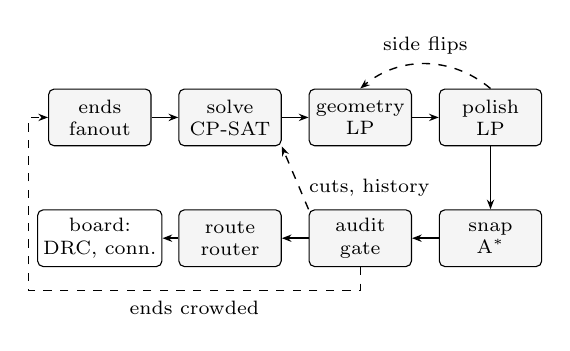
\begin{tikzpicture}[font=\scriptsize,node distance=0.8cm and 0.34cm,
  box/.style={draw,rounded corners=2pt,align=center,minimum height=0.72cm,minimum width=1.3cm,inner sep=2pt,fill=gray!8},
  fb/.style={-{Stealth[length=3.5pt]},dashed,line width=0.5pt},
  fw/.style={-{Stealth[length=3.5pt]},line width=0.6pt}]
\node[box] (e) {ends\\fanout};
\node[box,right=of e] (s) {solve\\CP-SAT};
\node[box,right=of s] (g) {geometry\\LP};
\node[box,right=of g] (p) {polish\\LP};
\node[box,below=of p] (n) {snap\\A$^*$};
\node[box,below=of g] (a) {audit\\gate};
\node[box,below=of s] (r) {route\\router};
\node[box,below=of e,fill=white] (c) {board:\\DRC, conn.};
\draw[fw] (e)--(s); \draw[fw] (s)--(g); \draw[fw] (g)--(p); \draw[fw] (p)--(n); \draw[fw] (n)--(a); \draw[fw] (a)--(r); \draw[fw] (r)--(c);
\draw[fb] (p.north) to[bend right=40] node[above]{side flips} (g.north);
\draw[fb] (a.north west) -- node[right,pos=0.35]{cuts, history} (s.south east);
\draw[fb] (a.south) -- ++(0,-0.3) -| node[pos=0.25,below]{ends crowded} ($(e.west)+(-0.25,0)$) -- (e.west);
\end{tikzpicture}
\caption{The whole route. Solid arrows pass the plan forward; dashed arrows are the negotiation: findings between the arrays return to the solve as cuts and history, lanes with no room beside an island return to the geometry as side flips, and findings at the ends return to the choice of escapes.}
\label{fig:loop}
\end{figure}

\section{Results}
\label{sec:results}
\subsection{Benches and grading}
\emph{H3.} An Allwinner H3 (0.65\,mm ball pitch) to a DDR3 device on a public reference design~\cite{h3board}, whose designer routed the bus on its two layers. Its bench carries 51 bus nets, among them three differential pairs (two data strobes and the clock); the ladder's rungs K15--K51 add whole groups of nets, tightest first.
\emph{Zynq.} The Zynq-7020 (CLG400) and its DDR3 on a public design~\cite{zynqboard}, whose designer routed the bus on the outer layers only (the inner layers are planes), 103 vias, every one F to B. We strip its routing, fan out the processor, and keep the two outer layers; the ladder runs to 44 nets with both strobe pairs.\TODO{re-run on the current bench build.}

Each result is written as a board and graded independently: connectivity of every bus net, DRC at the routed clearance of 0.1\,mm, and a census of every via and millimetre of the run's nets, stubs included. The human's copper on the same nets is counted the same way; it includes length-matching meanders, which add copper but no vias. Runs used CP-SAT from OR-Tools 9.15 and HiGHS through SciPy 1.16 on an Apple M3 laptop (8 cores, 8\,GB).

\begin{table}[t]
\centering
\caption{Vias / copper (mm) of the run's nets on the finished board, and the whole route's wall time and peak memory on an 8-core laptop running four rungs side by side (so wall time includes waiting). Every entry of the whole route is connected and DRC-clean at 0.1\,mm.}
\label{tab:results}
\setlength{\tabcolsep}{4.5pt}
\begin{tabular}{lcccc}
\toprule
rung & whole route & human & wall (s) & memory (MB) \\
\midrule
\multicolumn{5}{l}{\emph{Allwinner H3 to DDR3}} \\
K15 & \textbf{10} / 199 & 22 / 232 & 39 & 241 \\
K28 & \textbf{30} / 589 & 48 / 678 & 169 & 436 \\
K35 & \textbf{58} / 779 & 60 / 889 & 341 & 434 \\
K41 & \textbf{70} / 1040 & 70 / 1081 & 595 & 593 \\
K51 & \textbf{80} / 1220 & 88 / 1337 & 1295 & 720 \\
\midrule
\multicolumn{5}{l}{\emph{Zynq-7020 to DDR3}} \\
K18 & \textbf{12} / 466 & 45 / 662 & 139 & 404 \\
K26 & \textbf{30} / 732 & 57 / 923 & 412 & 464 \\
K32 & \textbf{46} / 940 & 74 / 1166 & 475 & 693 \\
K38 & \textbf{54} / 1121 & 86 / 1373 & 428 & 671 \\
K42 & \textbf{62} / 1263 & 97 / 1534 & 1892 & 842 \\
K44 & \textbf{58} / 1347 & 103 / 1617 & 767 & 769 \\
\bottomrule
\end{tabular}
\end{table}

\subsection{Against the human}
Table~\ref{tab:results} gives every rung of both ladders on our own ends. Every rung routes every lane in its band at once, every net connected, DRC-clean, never with more vias than the human and always with less copper. At the top of the H3 ladder the route uses 80 vias to the human's 88 (Fig.~\ref{fig:k51}); on the Zynq, 58 to 103. Part of the copper difference is the human's length matching; none of the via difference is.

On the human's own ends at K51---its teeth and berths clipped from its board---the whole route uses 88 vias to the human's 88, in 1263\,mm of copper to 1337. Our earlier approach, which routes corridors of lanes stage by stage from a CP-SAT plan of the ends and repairs refusals by rip-up, needed 101 vias on those ends, and on our own ends left five nets open at 144 vias.

\begin{figure*}[t]
\centering
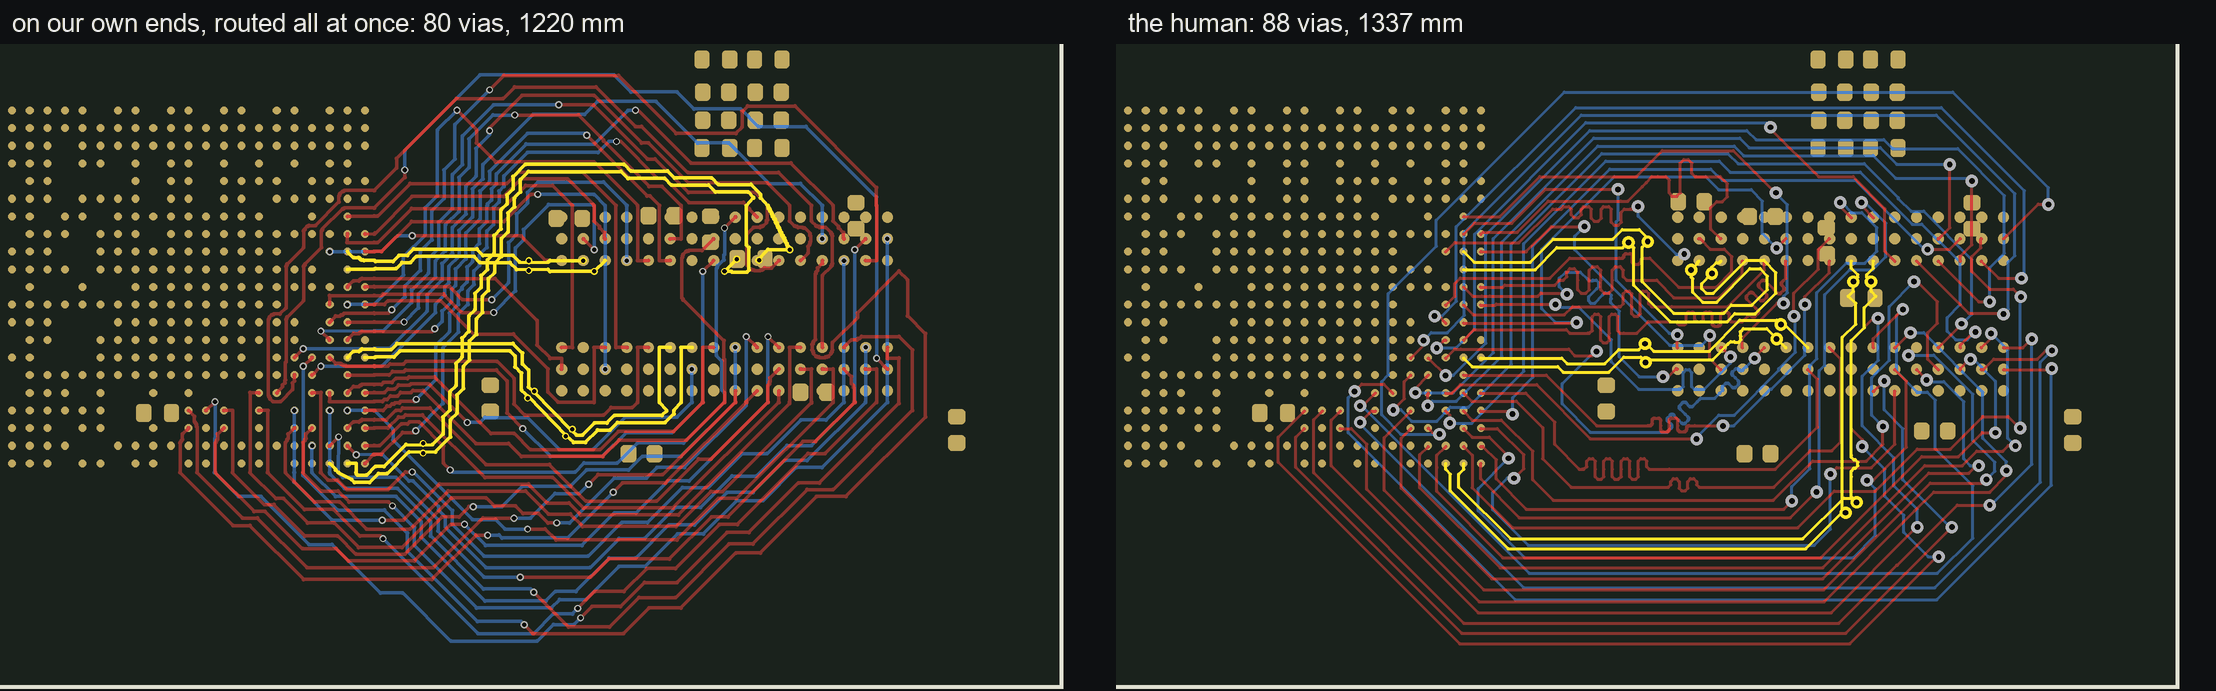
\includegraphics[width=0.86\textwidth]{figs/k51_own_ends.png}
\caption{The 51-net H3 rung. Left: our ends and the whole route, 80 vias and 1220\,mm. Right: the human's board on the same nets, 88 vias and 1337\,mm. F is red, B blue; the three differential pairs are yellow. The source BGA is at left, the DDR3 at right.}
\label{fig:k51}
\end{figure*}

\subsection{Cost}
Most of the time is spent choosing the ends: of K51's 1295\,s, the fanout with its exact re-ranking takes 829\,s, the first solve 25\,s, and one loop round under three minutes, half of it the geometry LP.\TODO{per-rung crossings, triples and solve times; an external baseline routed through the same router; the synthetic buses against their known optima.}

\section{Limitations and Future Work}
\label{sec:limits}
The route does not match lengths; a DDR interface requires length (or delay) matching within byte lanes and of the address group to the clock~\cite{ozdal2006length}, and the human's copper includes that work. Matching lengths on the planned lanes, where the comfortable pitch leaves room for meanders, is our next step. The model is for two signal layers; boards with more layers route the bus on more, and the model's spins become multi-valued. Optimality is relative to the model (fixed ends, reduced braids, at most three changes per lane, heuristic cuts), and the ends are chosen by a local search whose estimate is exact only in its parts; a single CP model over the ends could prove them. The solve counts a pair's dive once, where the board counts two barrels, so its equal optima can differ on the board by two vias. Intra-pair skew is not yet planned. Finally, two boards are few, and the design constants were developed on them; we are extending the evaluation to more boards and to synthetic buses with known optima.

\section{Conclusion}
Planning a bus whole---ends, crossings, their order and every layer change, decided at once, proved minimal in vias within the model, and negotiated with the geometry until the production router can lay it---routes two real DDR3 buses fully automatically, with fewer vias than their designers. The central model is small and exact because the problem's combinatorics are those of a wiring diagram, whose consistency is a rule over triples. We hope the benches, which are public, give later work a way to compare against finished copper and against the human. Throughout this work the synergies between routing and physics proved abundant, interesting and of practical use: the worldline picture gives the triple rule its meaning, the spin picture traces every via to frustration, and the forces of the linear program's dual name the rules that hold each lane and the ones that must yield. We expect the same pairing---an exact choice of topological sector, relaxed in a convex statics problem whose forces steer the next choice---to carry over to length matching, to boards with more layers and to the other dense interconnects of modern hardware, and the dialogue between routing and physics to keep paying in both directions.

\section*{Acknowledgment}
In accordance with IEEE policy, the author discloses that portions of the software were drafted with the assistance of an AI system (Claude, Anthropic); the author reviewed and takes responsibility for all content.

\bibliographystyle{IEEEtran}
\bibliography{refs}

\end{document}
